% ------------------------------------------------------------------------------
% TYPO3 Version 9.4 - What's New (French Version)
%
% @license	Creative Commons BY-NC-SA 3.0
% @link		https://typo3.org/help/documentation/whats-new/
% @language	French
% ------------------------------------------------------------------------------

\section{Interface Utilisateur Backend}
\begin{frame}[fragile]
	\frametitle{Interface Utilisateur Backend}

	\begin{center}\huge{Chapitre 1~:}\end{center}
	\begin{center}\huge{\color{typo3darkgrey}\textbf{Interface Utilisateur Backend}}\end{center}

\end{frame}

% ------------------------------------------------------------------------------
% Admin Panel (1)

\begin{frame}[fragile]
	\frametitle{Interface Utilisateur Backend}
	\framesubtitle{Panneau d'administration (1)}

    Le panneau d'administration a reçu une rénovation complète concernant son
    apparence ainsi que son architecture et le code sous-jacent.
	\newline\newline
	Le Panneau d'administration est affiché en bas des pages du frontend de TYPO3.
	L'interrupteur à sa droite permet son activation et sa désactivation par les
	intégrateurs et les contributeurs. Son état actuel montre l'état d'\textit{activation}.

	\begin{figure}
		
\includegraphics[width=0.90\linewidth]{BackendUserInterface/AdminPanelEnabled.png}
	\end{figure}

\end{frame}

% ------------------------------------------------------------------------------
% Admin Panel (2)

\begin{frame}[fragile]
	\frametitle{Interface Utilisateur Backend}
	\framesubtitle{Panneau d'administration (2)}

	La capture d'exemple ci-dessous montre les options TypoScript.

	\begin{figure}
		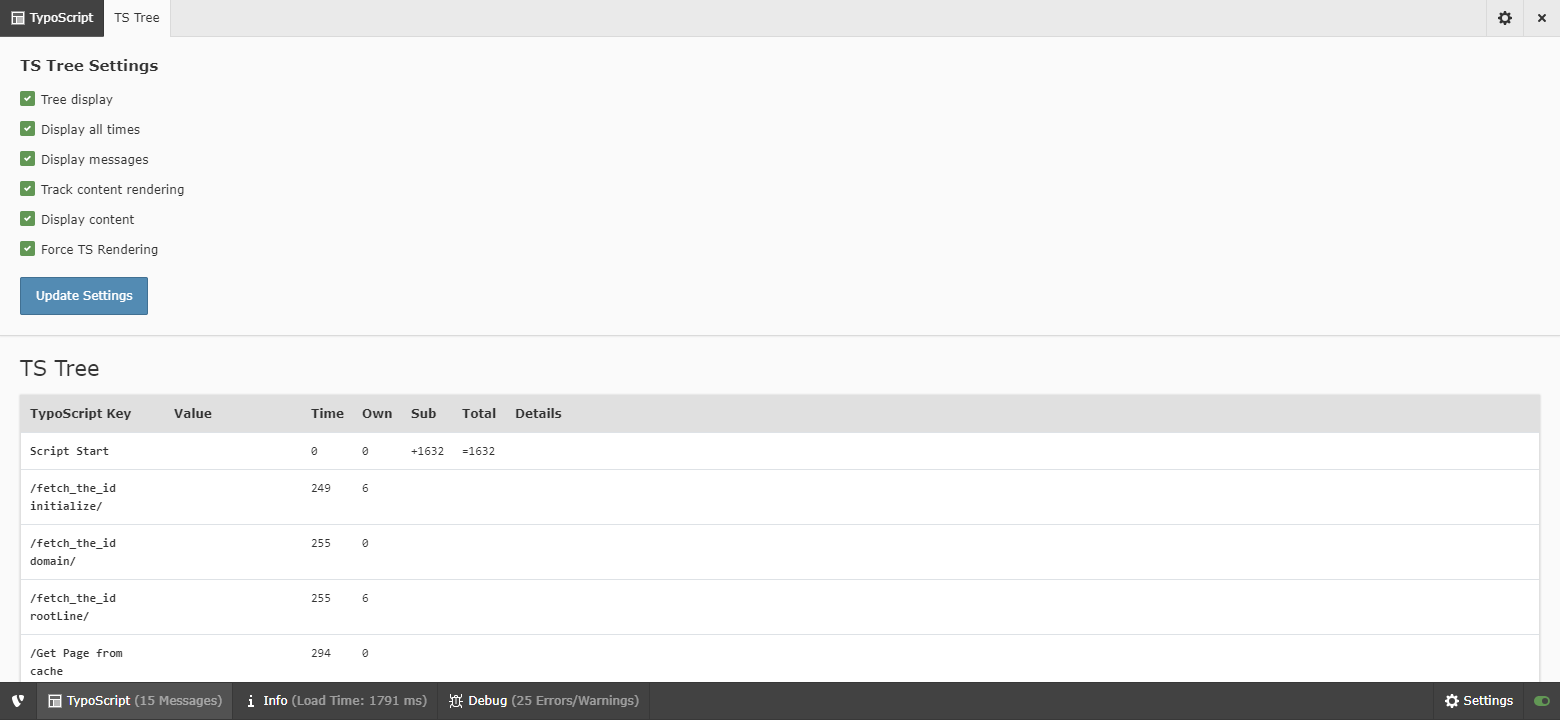
\includegraphics[width=0.90\linewidth]{BackendUserInterface/AdminPanelTypoScript.png}
	\end{figure}

\end{frame}

% ------------------------------------------------------------------------------
% Admin Panel (3)

\begin{frame}[fragile]
	\frametitle{Interface Utilisateur Backend}
	\framesubtitle{Panneau d'administration (3)}

	La capture d'exemple ci-dessous montre les options de configuration («~Settings~»).

	\begin{figure}
		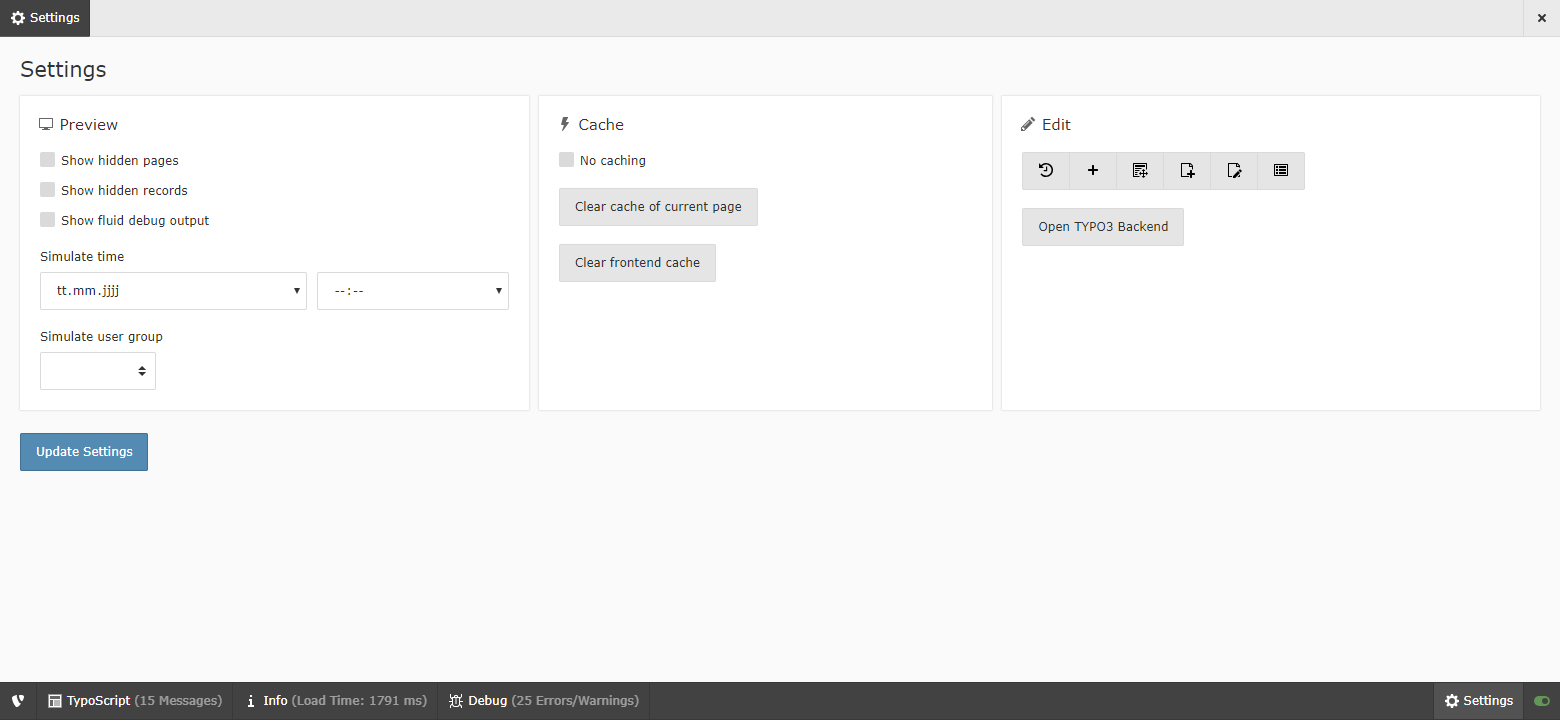
\includegraphics[width=0.90\linewidth]{BackendUserInterface/AdminPanelSettings.png}
	\end{figure}

\end{frame}

% ------------------------------------------------------------------------------
% #85398 - EXT:documentation removed

\begin{frame}[fragile]
	\frametitle{Interface Utilisateur Backend}
	\framesubtitle{L'extension «~Documentation~» retirée}

	Le module «~Documentation~» est retiré du backend de TYPO3.
	Le module possédait des défauts techniques et conceptuels. L'adoption
	par la communauté était faible.
    \newline
    Toutes les documentations restent disponibles à \href{https://docs.typo3.org}{docs.typo3.org}.

	\begin{figure}
		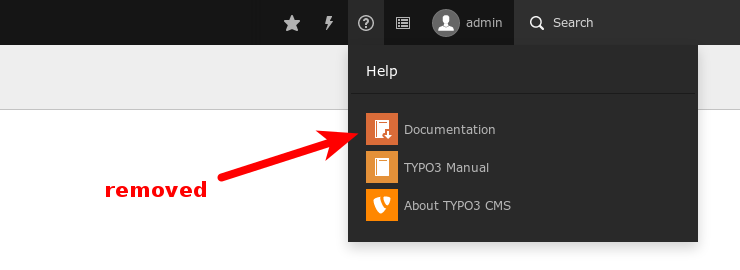
\includegraphics[width=0.70\linewidth]{BackendUserInterface/85398-ExtensionDocumentationRemoved.png}
	\end{figure}

\end{frame}

% ------------------------------------------------------------------------------
% #13265 - Select first element of page tree toolbar on initialization

\begin{frame}[fragile]
	\frametitle{Interface Utilisateur Backend}
	\framesubtitle{Barre d'outils de l'arborescence}

	Le premier élément de la barre d'outils de l'arborescence des page est maintenant
	sélectionné au chargement.

	\begin{figure}
		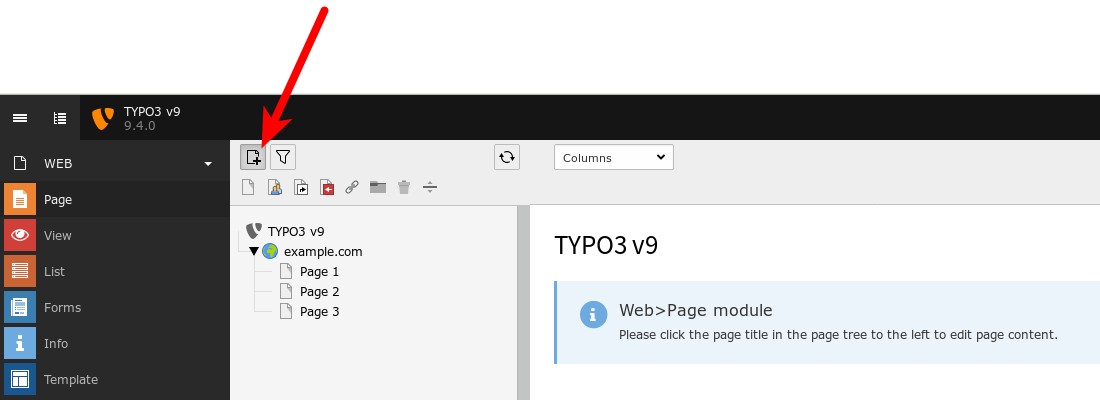
\includegraphics[width=0.90\linewidth]{BackendUserInterface/13265-FirstElementOfPageTree.png}
	\end{figure}

\end{frame}

% ------------------------------------------------------------------------------
% #85313 - Add notes field to pages table

\begin{frame}[fragile]
	\frametitle{Interface Utilisateur Backend}
	\framesubtitle{Notes pour les pages}

	Dans le nouvel onglet «~Notes~», un champ «~description~» est fourni. Il
	permet aux utilisateurs d'ajouter des notes. Les autres utilisateurs
	peuvent voir et éditer celles-ci.

	\begin{figure}
		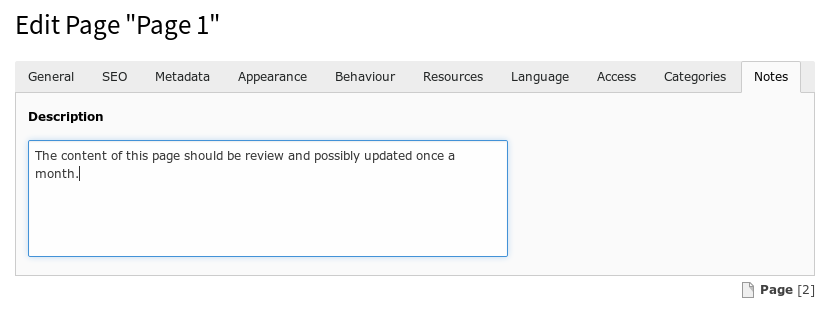
\includegraphics[width=0.90\linewidth]{BackendUserInterface/85313-NotesFieldForPages.png}
	\end{figure}

\end{frame}

% ------------------------------------------------------------------------------
% #xxxxx - Languages Visible in Frontend

\begin{frame}[fragile]
	\frametitle{Interface Utilisateur Backend}
	\framesubtitle{Langues définies uniquement}

	Les langues du site web dans le backend sont restreintes à celles définies
	sous «~Site Management → Site Configuration → Languages~». Il est possible
	de les activer/désactiver séparément.

	\begin{figure}
		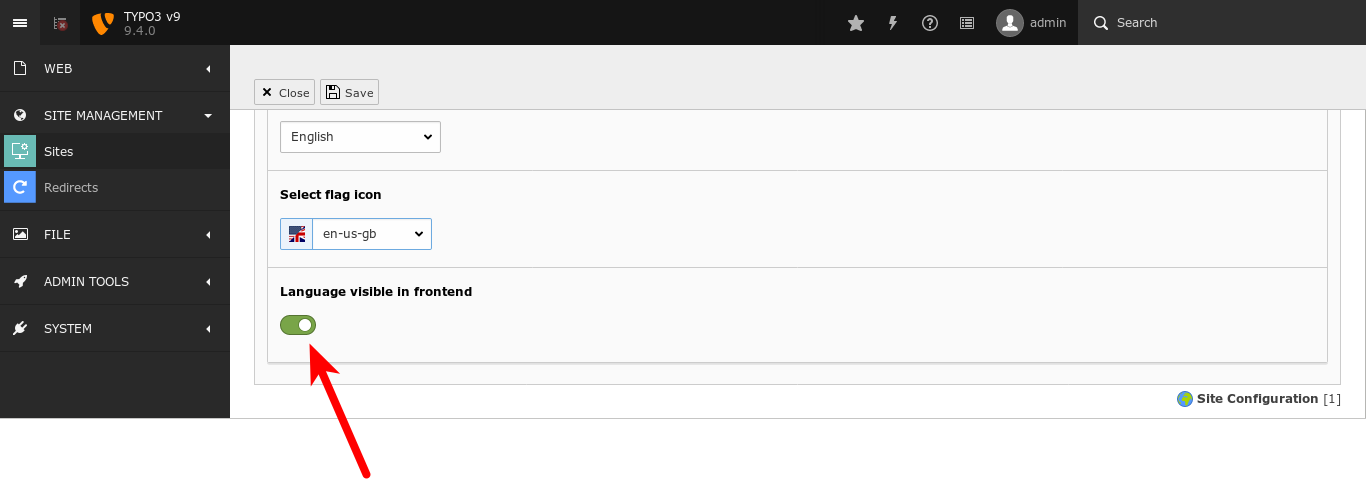
\includegraphics[width=0.90\linewidth]{BackendUserInterface/xxxxx-LanguagesVisibleInFrontend.png}
	\end{figure}

\end{frame}

% ------------------------------------------------------------------------------
% #85691 - Show page path in record info

\begin{frame}[fragile]
	\frametitle{Interface Utilisateur Backend}
	\framesubtitle{Chemin vers la page dans les informations d'enregistrement}

	Les indications de références des enregistrements incluent le chemin dans l'arborescence.

	\begin{figure}
		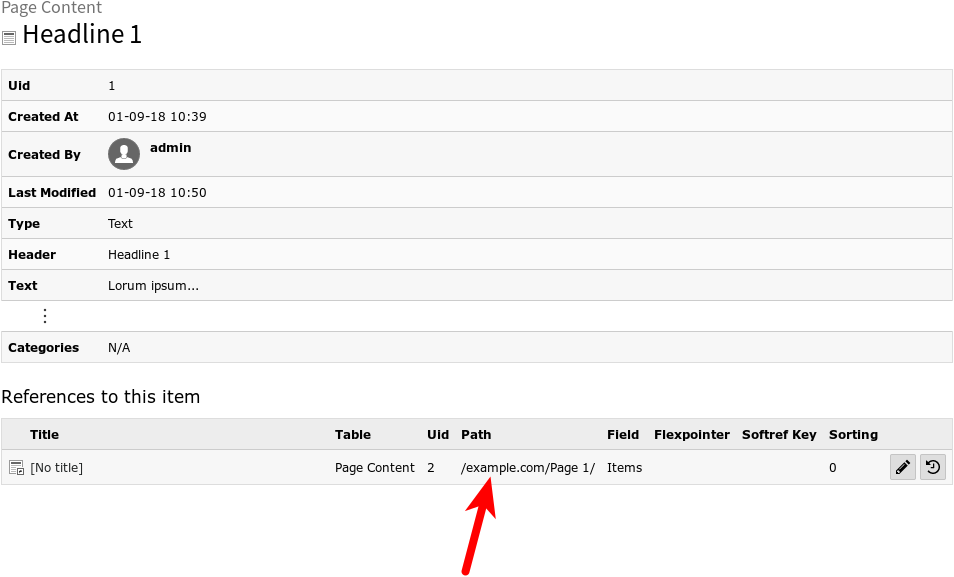
\includegraphics[width=0.70\linewidth]{BackendUserInterface/85691-ShowPagePathInRecordInfo.png}
	\end{figure}

\end{frame}

% ------------------------------------------------------------------------------
% Page-based URL Handling (aka "URL Routing")

\begin{frame}[fragile]
	\frametitle{Interface Utilisateur Backend}
	\framesubtitle{Gestion des URL des pages}

 	Le support natif du routage des URL de page est ajouté.

	\begin{figure}
		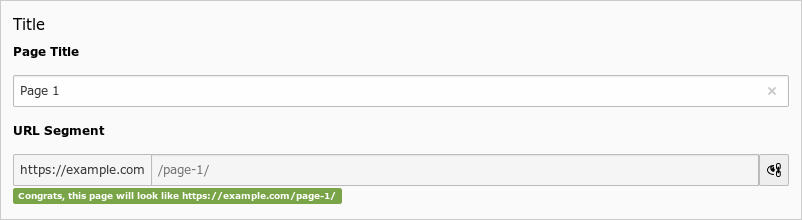
\includegraphics[width=0.90\linewidth]{BackendUserInterface/xxxxx-UrlRouting.png}
	\end{figure}

\end{frame}

% ------------------------------------------------------------------------------
% Modal Windows

% %%%%%%%%%%%%%%%%%%%%%%%%%%%%%%%%%%%%%%%%%%%%%%%%%%%%%%%%%%%%%% %
% Let's do not mention this in v9.4, but in v9.5 (TYPO3 v9 LTS). %
% We aim to achieve that all(!) popups use modal windows by the  %
% release of v9 LTS.                                             %
% %%%%%%%%%%%%%%%%%%%%%%%%%%%%%%%%%%%%%%%%%%%%%%%%%%%%%%%%%%%%%% %

%\begin{frame}[fragile]
%	\frametitle{Interface Utilisateur Backend}
%	\framesubtitle{Modal Windows}
%
%	Almost all popup windows in the backend of TYPO3 are now "modal windows"
%	rather than small browser windows, which open.
%
%\end{frame}

% ------------------------------------------------------------------------------
